\section{Presentation of experimental or analytical results/descriptions of final constructed product}
在这一节我们主要讨论模型的测试结果和模型进一步改进的空间。


\subsection{带入测试集验证准确度}

在这里我们将训练好的模型应用到测试集上,计算模型的准确度。

\autoref{tab:model_accuracy}是模型在测试集上的准确度:(准确度定义为标签与模型预测一致的样本数占总样本数的比例)

\begin{table}
\centering
\caption{model accuracy on test set}
\begin{tabular}{cccccc}
    \toprule
    & normal & horizental\_line & vertical\_line & slope & other \\
    \midrule
    accuracy(\%) & 98.4 & 95.6 & 80.0 & 96.1 & 95.2 \\
    \bottomrule
\end{tabular}
\label{tab:model_accuracy}
\end{table}

可见,模型预测结果在normal上表现较好,而在vertical\_line上表现较差。这可能是由于用于测试的样本量较少,导致模型学习不足,难以判断。


\subsection{判断最佳切削角度}

在这里采用模型3d(inceptionv3)来判断最佳切削角度。我们将模型应用到测试集上,计算在每个切削角度下可用样本的占比。找到可用样本占比最多的区间,即为最佳切削角度。

\begin{table}
    \centering
    \caption{normal accuracy on different angle}
    \begin{tabular}{cccccccccc}
        \toprule
        & 8 & 8.5 & 9 & 9.5 & 10 & 10.5 & 11 & 11.5 & 12 \\
        \midrule
        accuracy(\%) & 80 & 81.5 & 83.5 & 93.3 & 96.6 & 88.8 & 84.2 & 66.6 & 62.2 \\ 
        \bottomrule
    \end{tabular}
    \label{tab:model_accuracy_angle}
    \end{table}

    由\autoref{tab:model_accuracy_angle}可知,最佳切削角度为10度。

    若要在保证切削质量为百分之80的情况下,切削角度应在9度到10.5度之间。


\subsection{模型的进一步提高(改变输入分辨率)(数据增强在这里)}

在这里我们讨论模型的进一步提高的空间。
在上文提到,在模型3d中的输入层是299*299的图片,而在实际应用中,特别是采集到的分辨率往往较高(如vhx7000则是2880*2160),将其重缩放为299*299可能会导致信息和细节丢失的情况。因此,我们可以考虑将模型的输入层改为更大的图片,以提高模型的准确度。并且因为InceptionV3模型的结构复杂,他对于大图片的处理能力较强,更加得心应手。

受制于实验室机器性能,在这里将图像缩放到分别为原图像的0.4倍,即1152*864,进行再一次训练。

新的模型为model4,训练效果如下所示:

\begin{figure}
    \centering
    \begin{minipage}{0.45\textwidth}
        \centering
        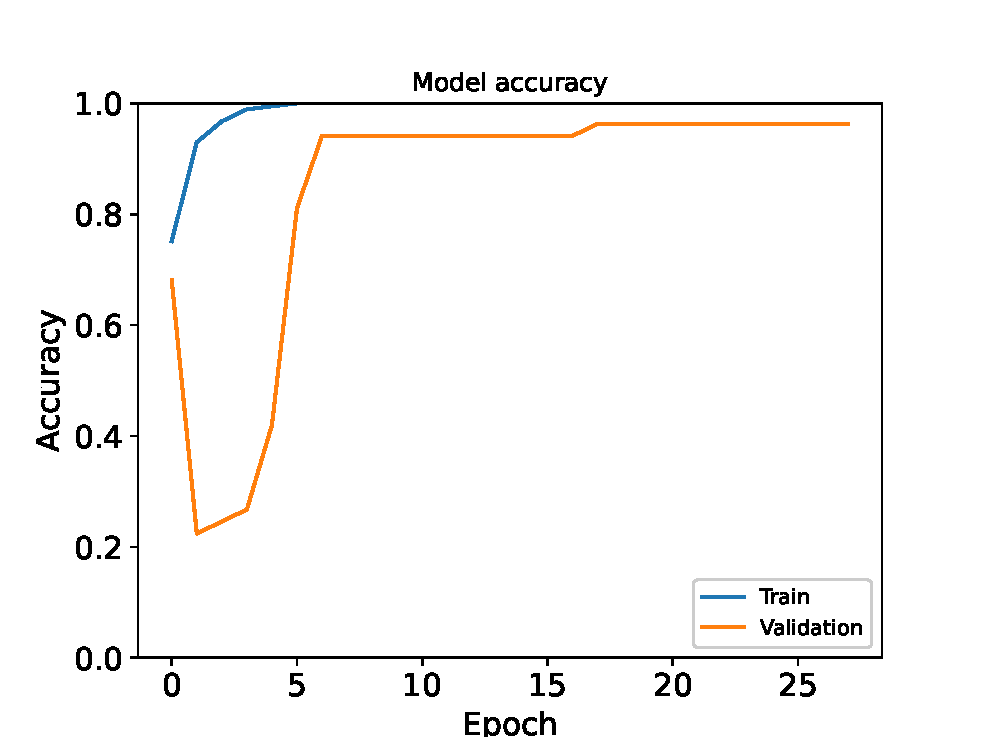
\includegraphics[width=\textwidth]{./fig/model4/accuracy4.eps}
        \caption{Model-4 accuracy}
        \label{fig:model4_accuracy}
    \end{minipage}
    \begin{minipage}{0.45\textwidth}
        \centering
        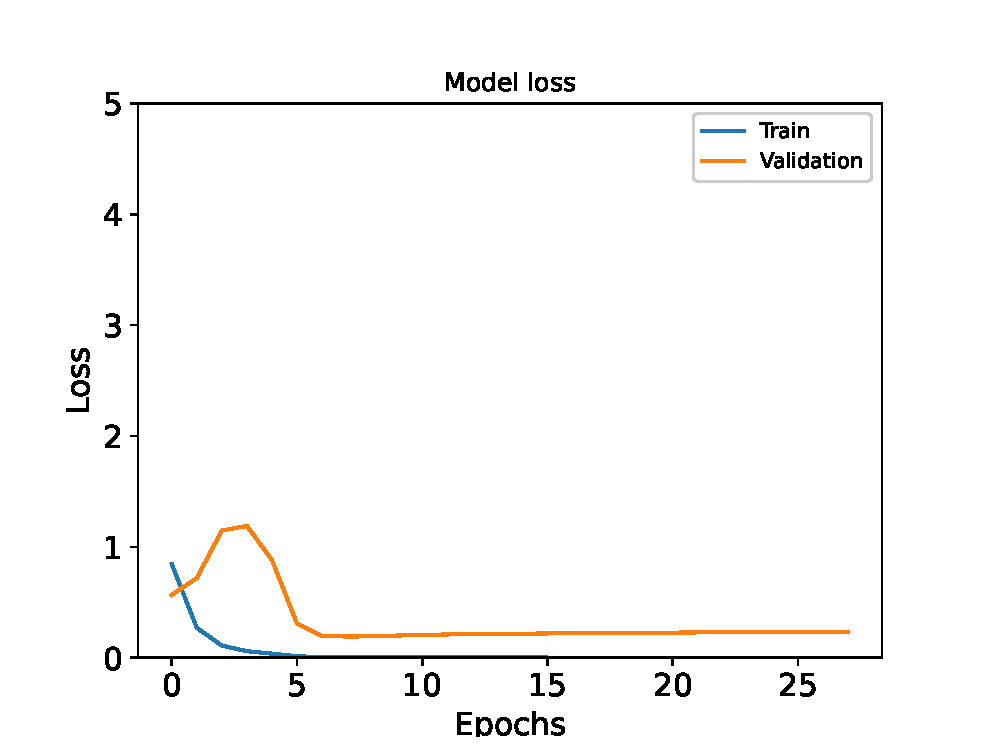
\includegraphics[width=\textwidth]{./fig/model4/loss4.eps}
        \caption{Model-4 loss}
        \label{fig:model4_loss}
    \end{minipage}
\end{figure}

观察训练准确度和损失随步长的变化可以发现,模型的性能有惊人的明显提升。其训练和验证准确度都已经逼近于1,验证集的损失也下降至0.2左右。这说明模型的泛化能力较强,可以很好地适应新的数据。


将其再一次带入测试集进行准确度评估,结果如\autoref{tab:model_accuracy2}:

\begin{table}
    \centering
    \caption{model accuracy on test set}
    \begin{tabular}{cccccc}
        \toprule
        & normal & horizental\_line & vertical\_line & slope & other \\
        \midrule
        accuracy(\%) & 98.4 & 96.7 & 85.6 & 96.5 & 96.5 \\
        \bottomrule
    \end{tabular}
    \label{tab:model_accuracy2}
    \end{table}

    对比修改分辨率前后的模型准确度,可以发现模型的准确度虽有提升但并不显著的,可能是由于准确度已经很接近于1,提升的空间较小导致的。


\subsection{模型通用性}

在上文的实验中我们采用的是鱼的卵巢为组织切片,而在实际应用中,我们可能会遇到其他组织切片,如其他器官或其他动物标本等。因此,我们需要考虑模型的通用性。

在这里有另一组已经采集好的数据集,是鱼的肺切片,一共分成4类,分别是good, normal, bad,other 四类(样本如\autoref{fig:good_fish_lung}到\autoref{fig:other_fish_lung})。现在更改输入数据集,保持原有模型架构不变,采用1152*864(0.4倍长宽)分辨率图片作为输入数据进行训练。

\begin{figure}
    \centering
    \begin{minipage}{0.45\textwidth}
        \centering
        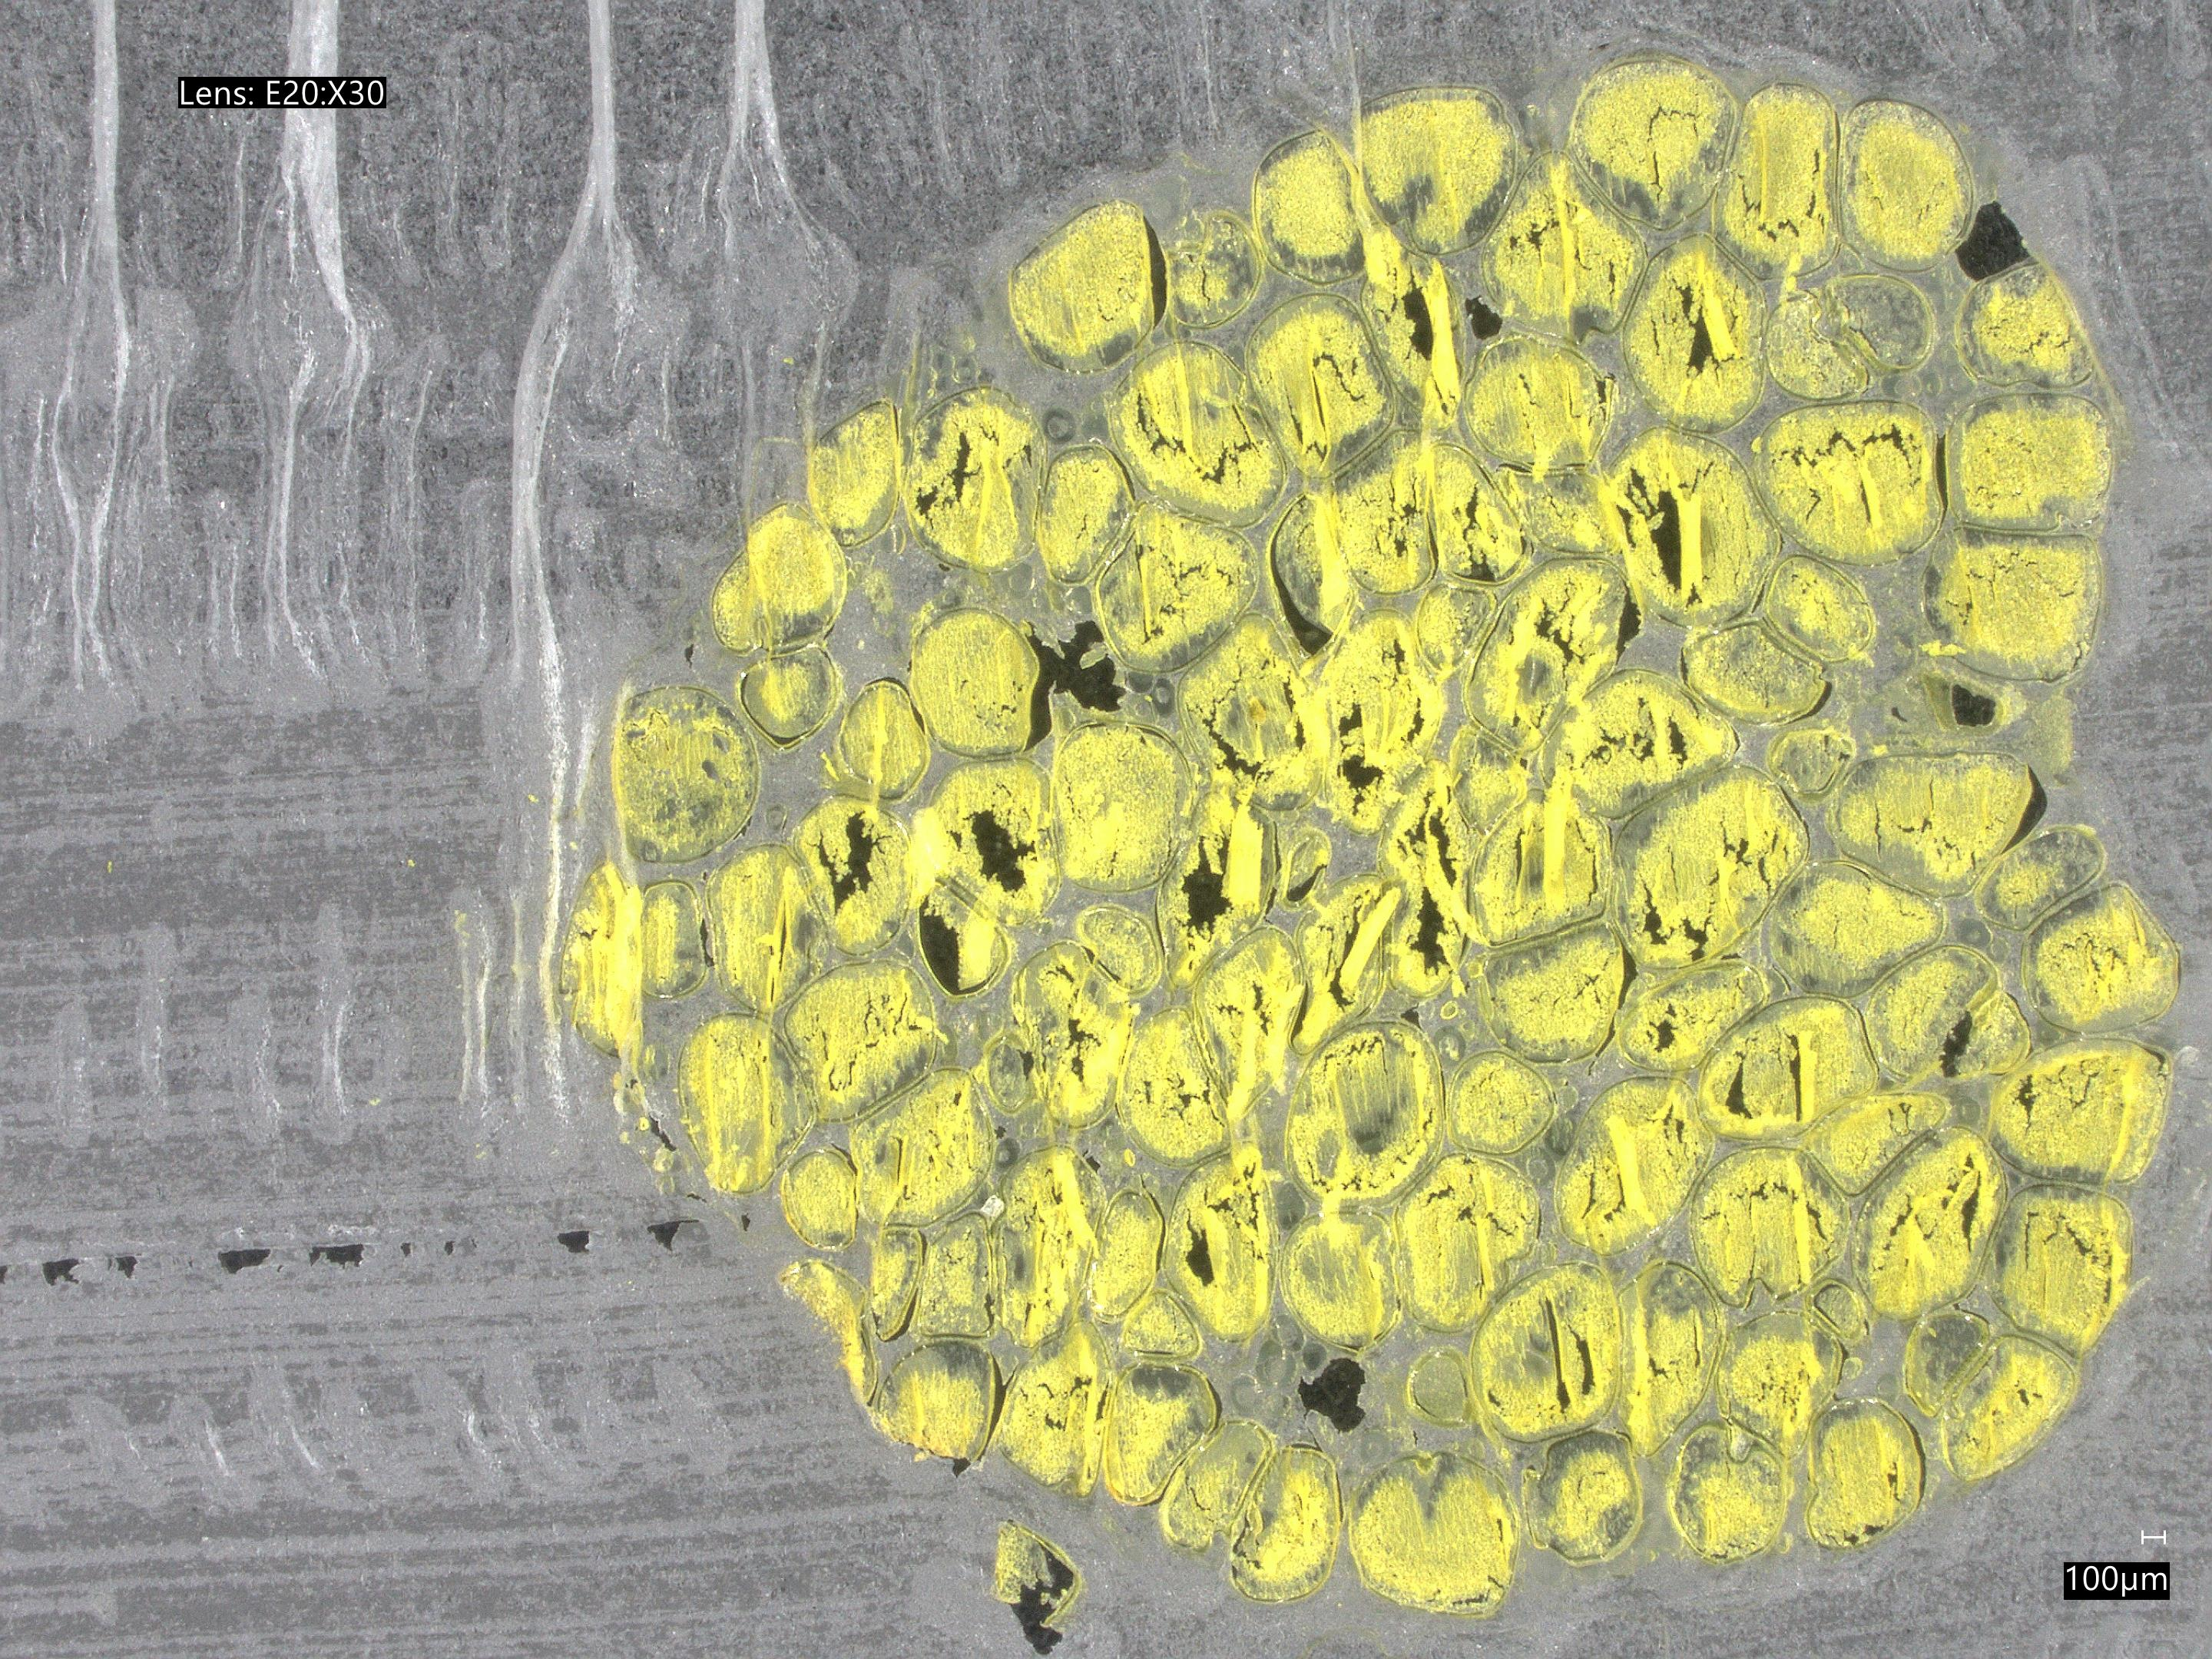
\includegraphics[width=\textwidth]{./fig/fish_lung/good20240313_144138.jpg}
        \caption{good fish lung}
        \label{fig:good_fish_lung}
    \end{minipage}
    \begin{minipage}{0.45\textwidth}
        \centering
        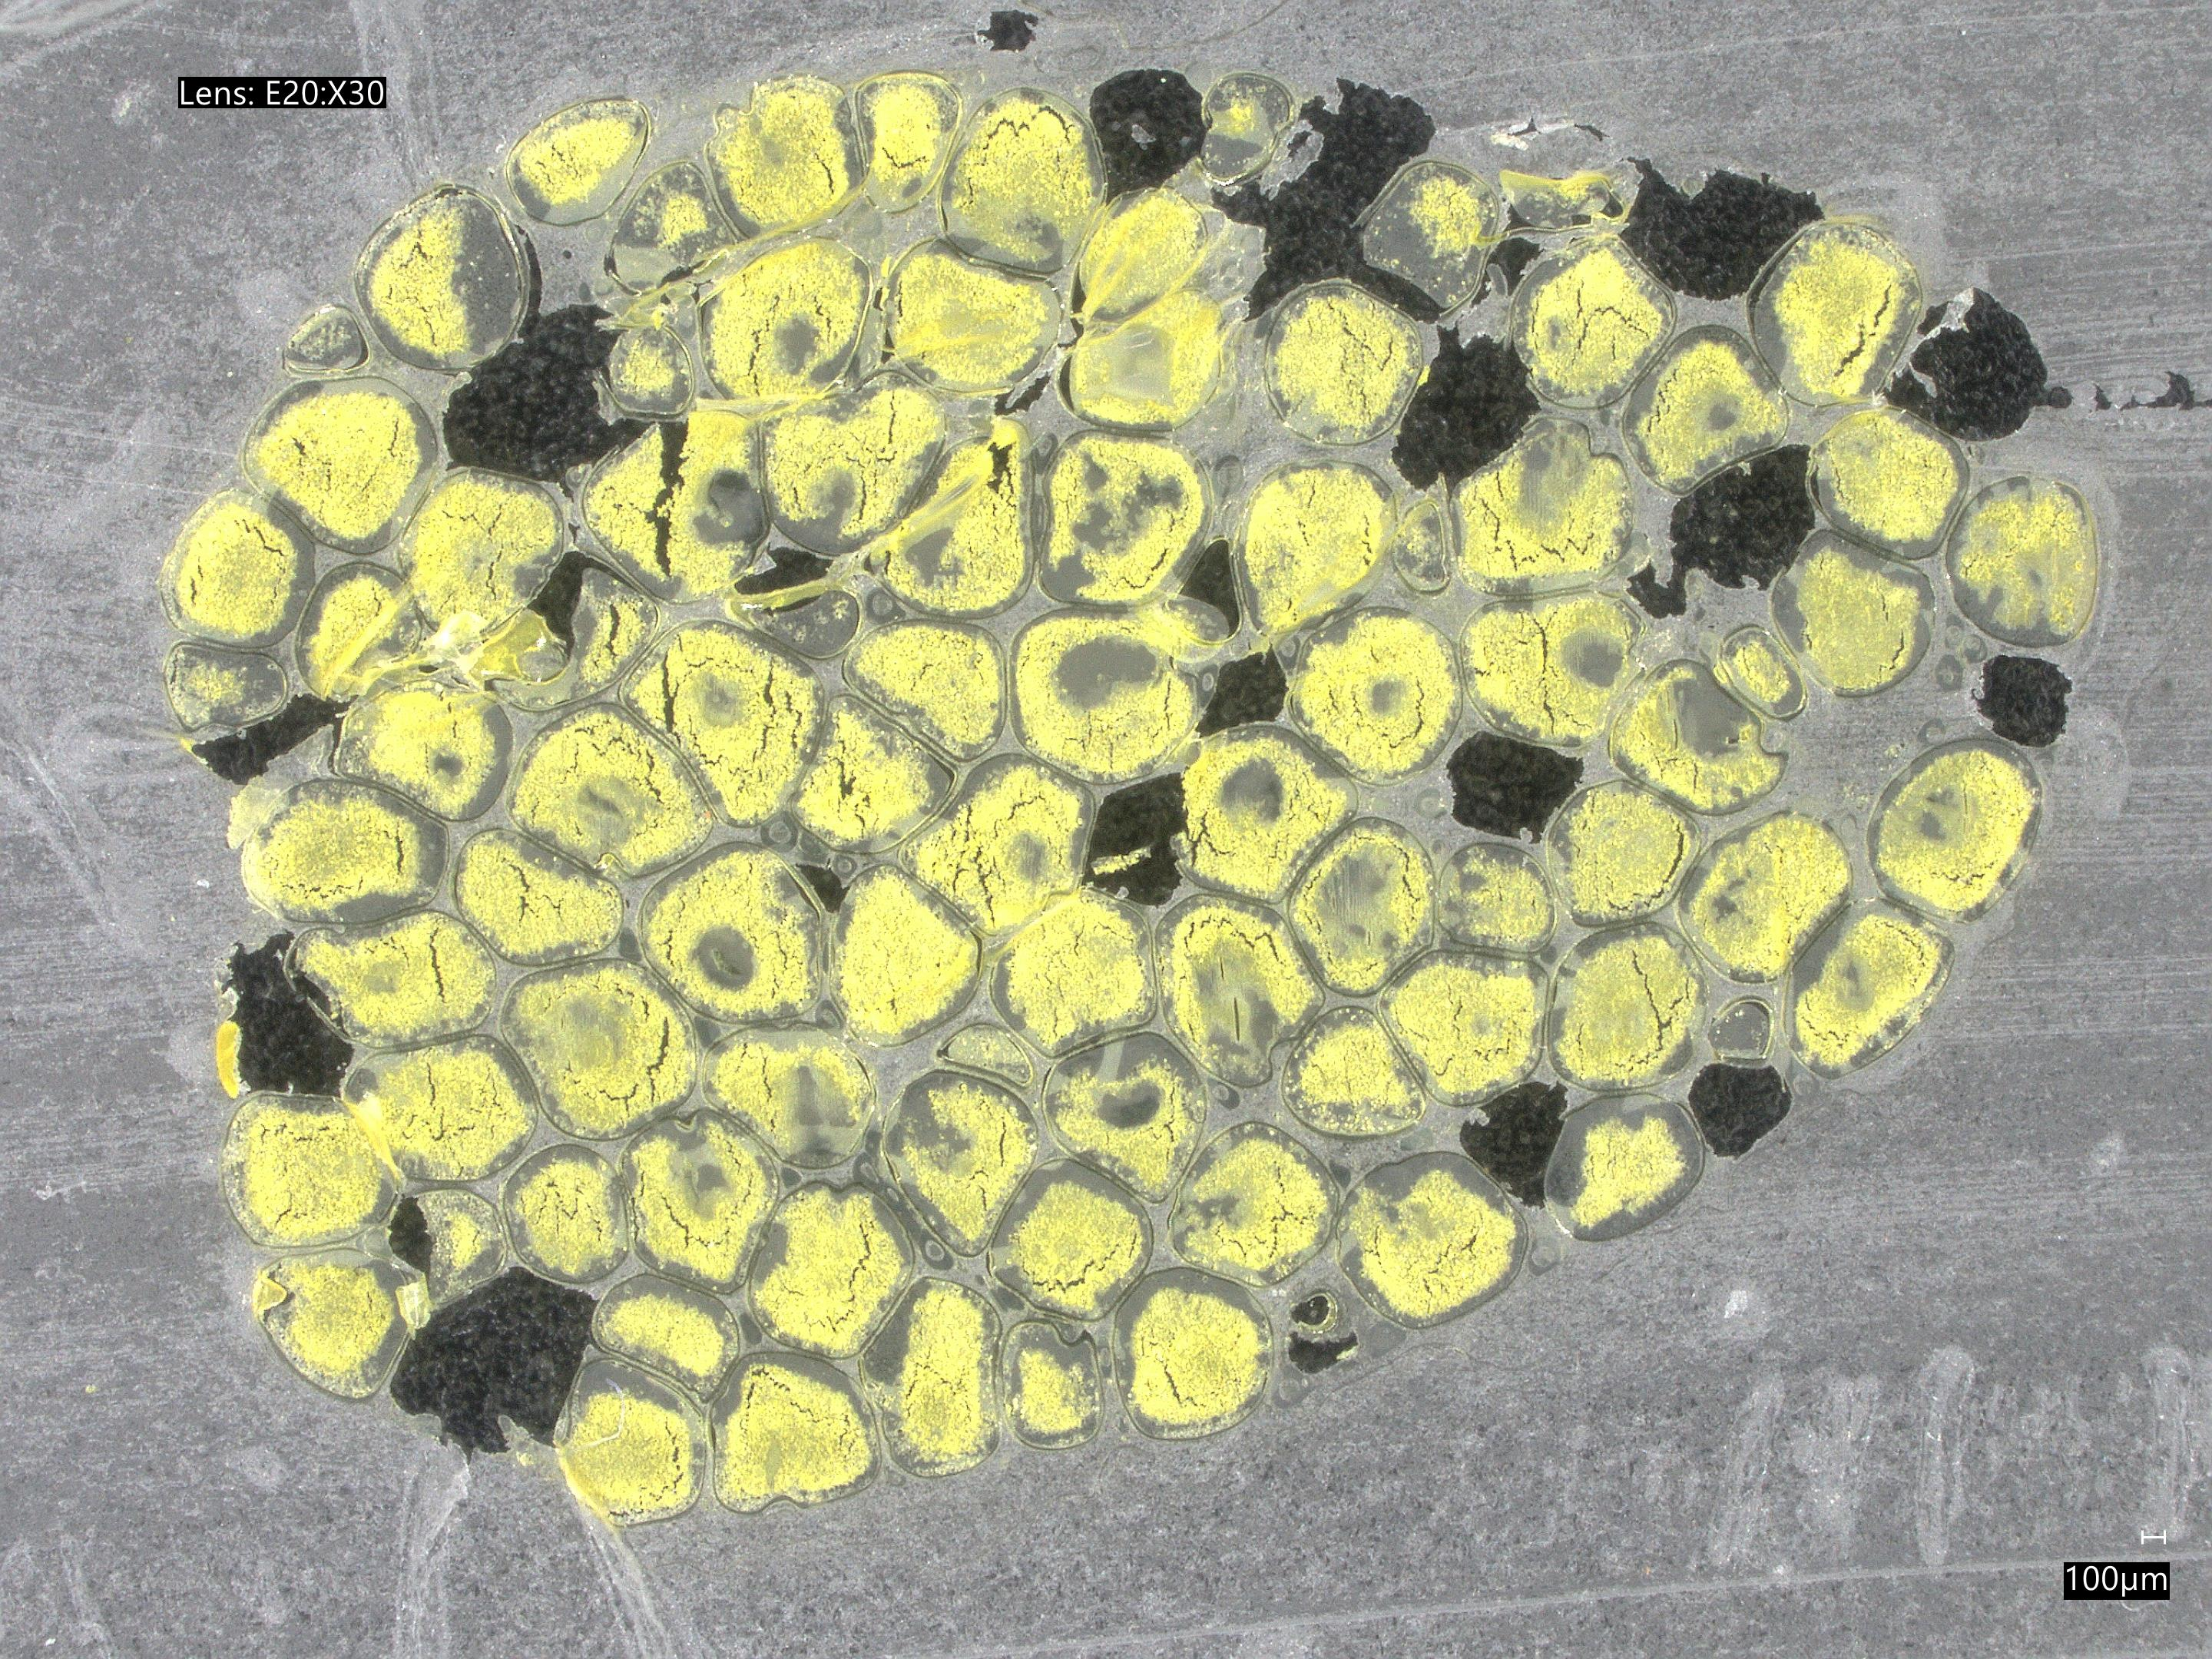
\includegraphics[width=\textwidth]{./fig/fish_lung/normal20240313_141726.jpg}
        \caption{normal fish lung}
        \label{fig:noraml_fish_lung}
    \end{minipage}
\end{figure}

\begin{figure}
    \centering
    \begin{minipage}{0.45\textwidth}
        \centering
        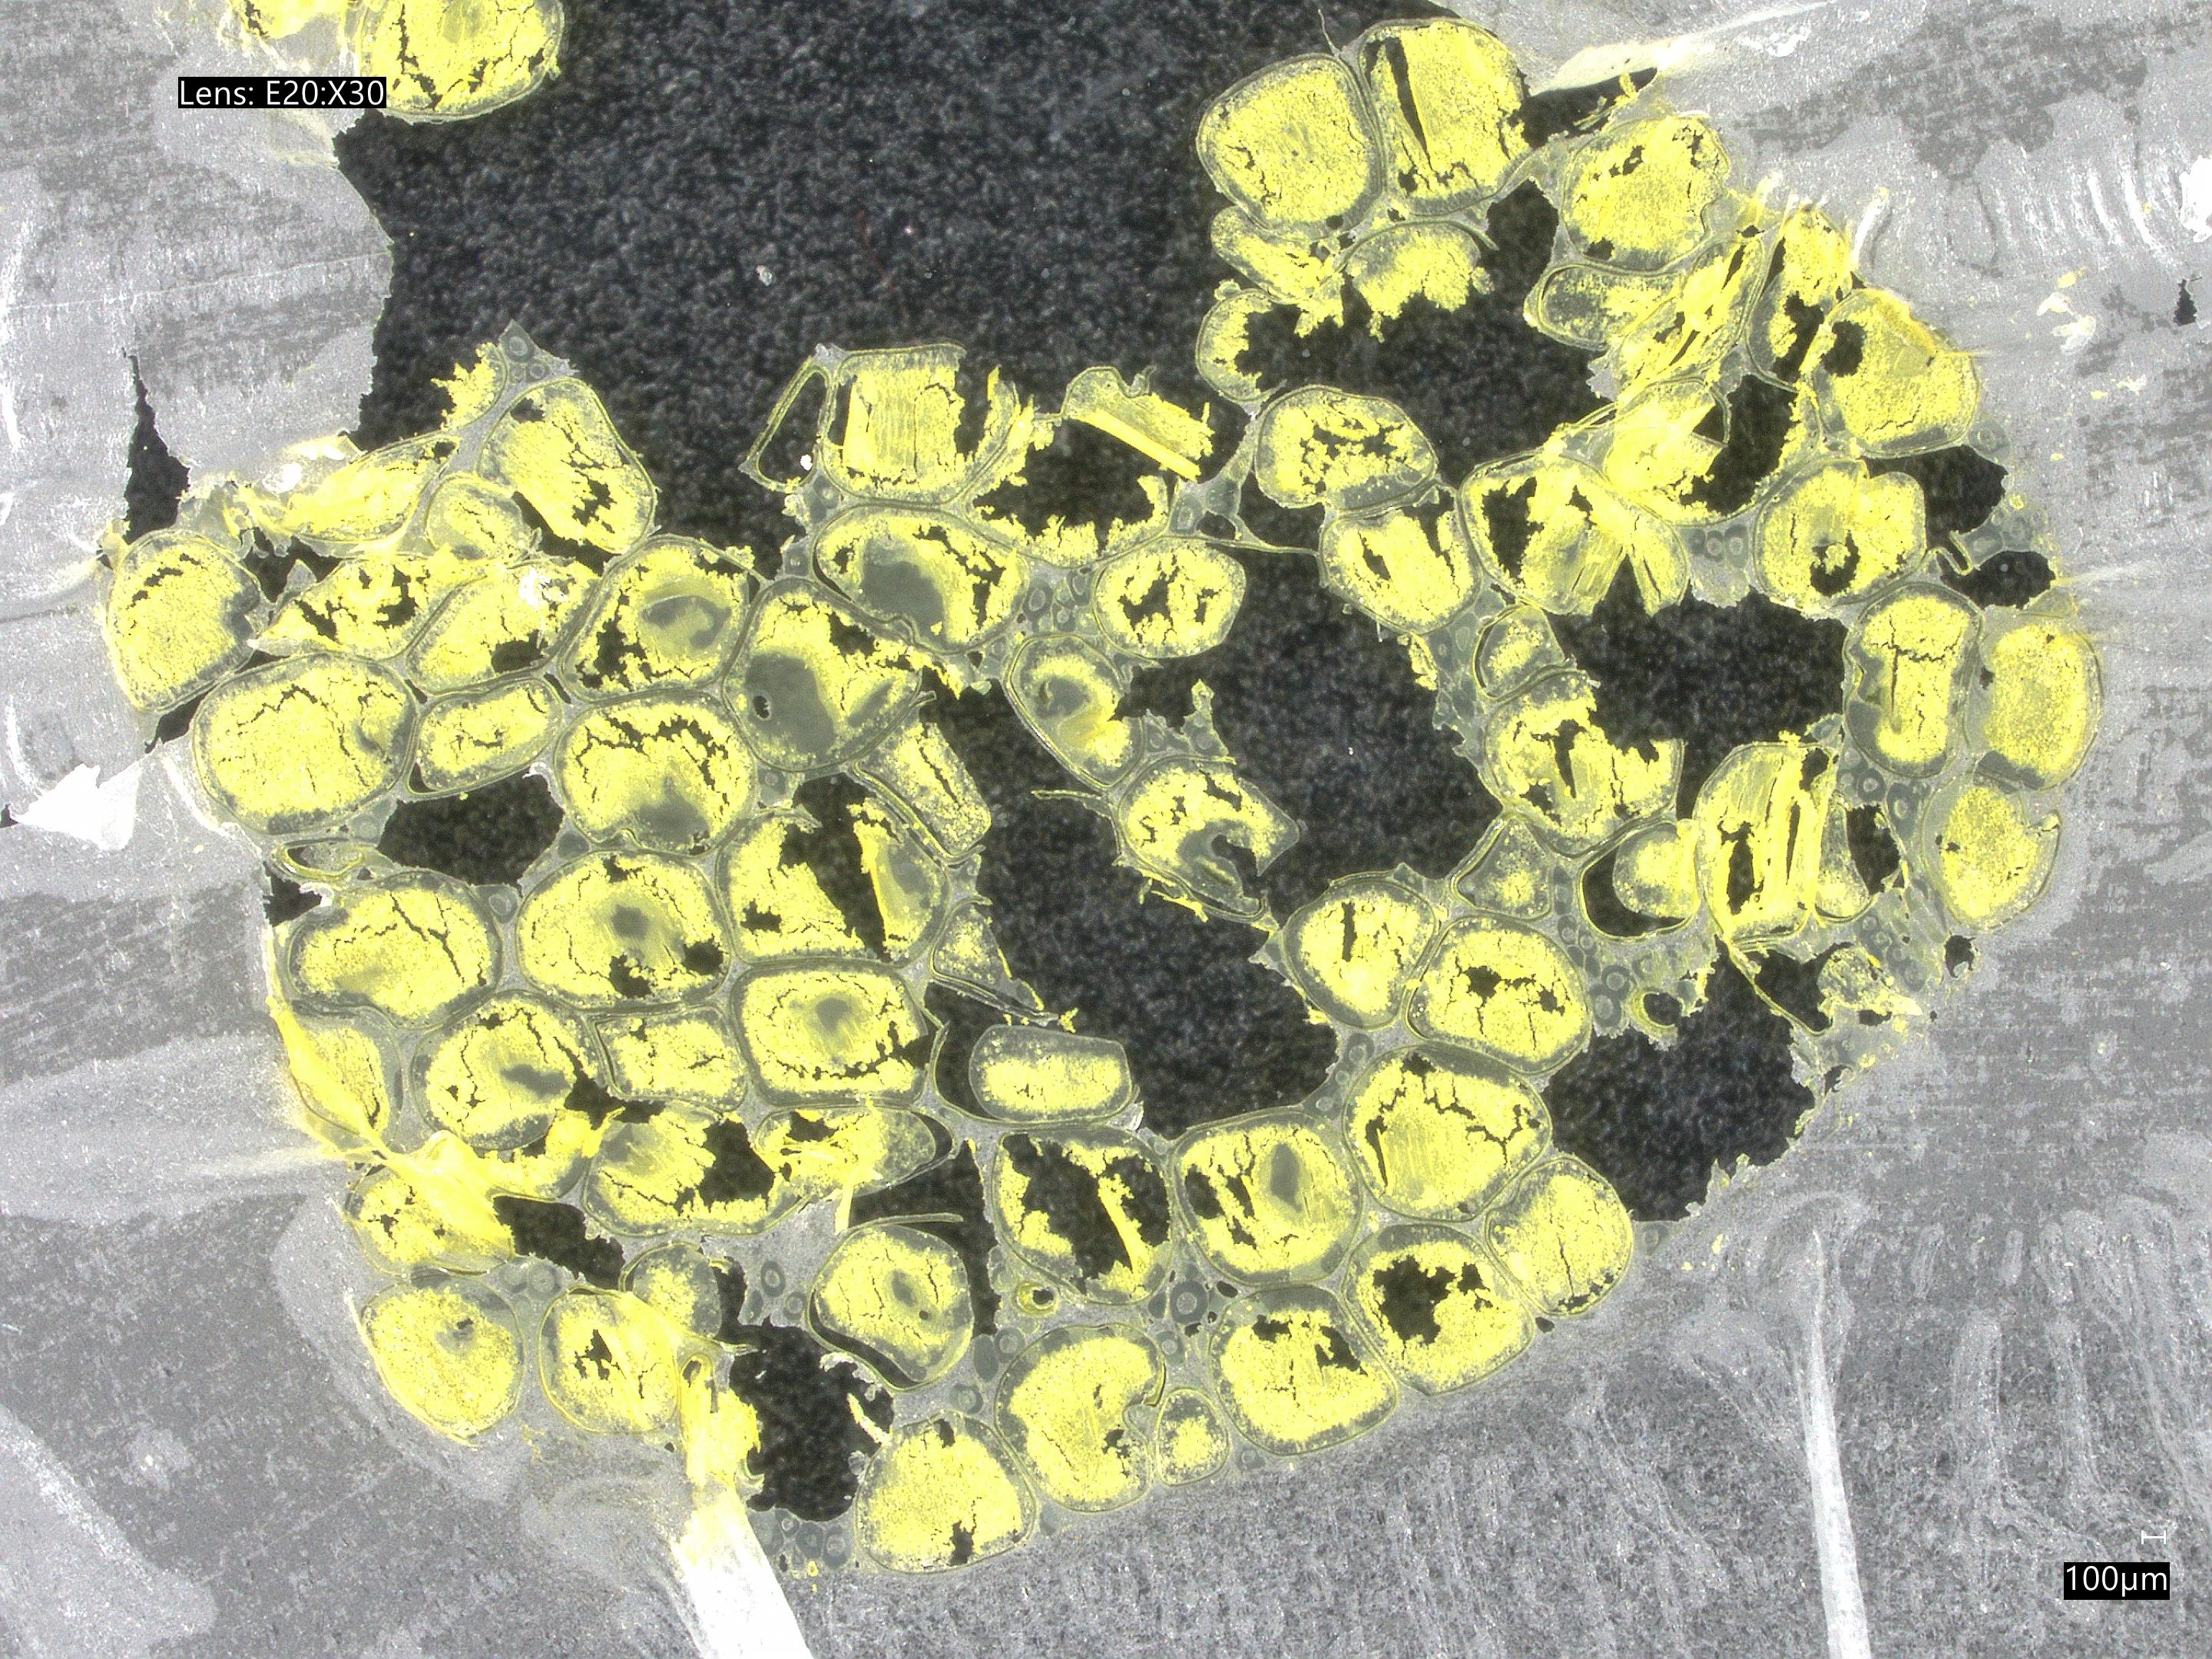
\includegraphics[width=\textwidth]{./fig/fish_lung/bad20240313_140952.jpg}
        \caption{bad fish lung}
        \label{fig:bad_fish_lung}
    \end{minipage}
    \begin{minipage}{0.45\textwidth}
        \centering
        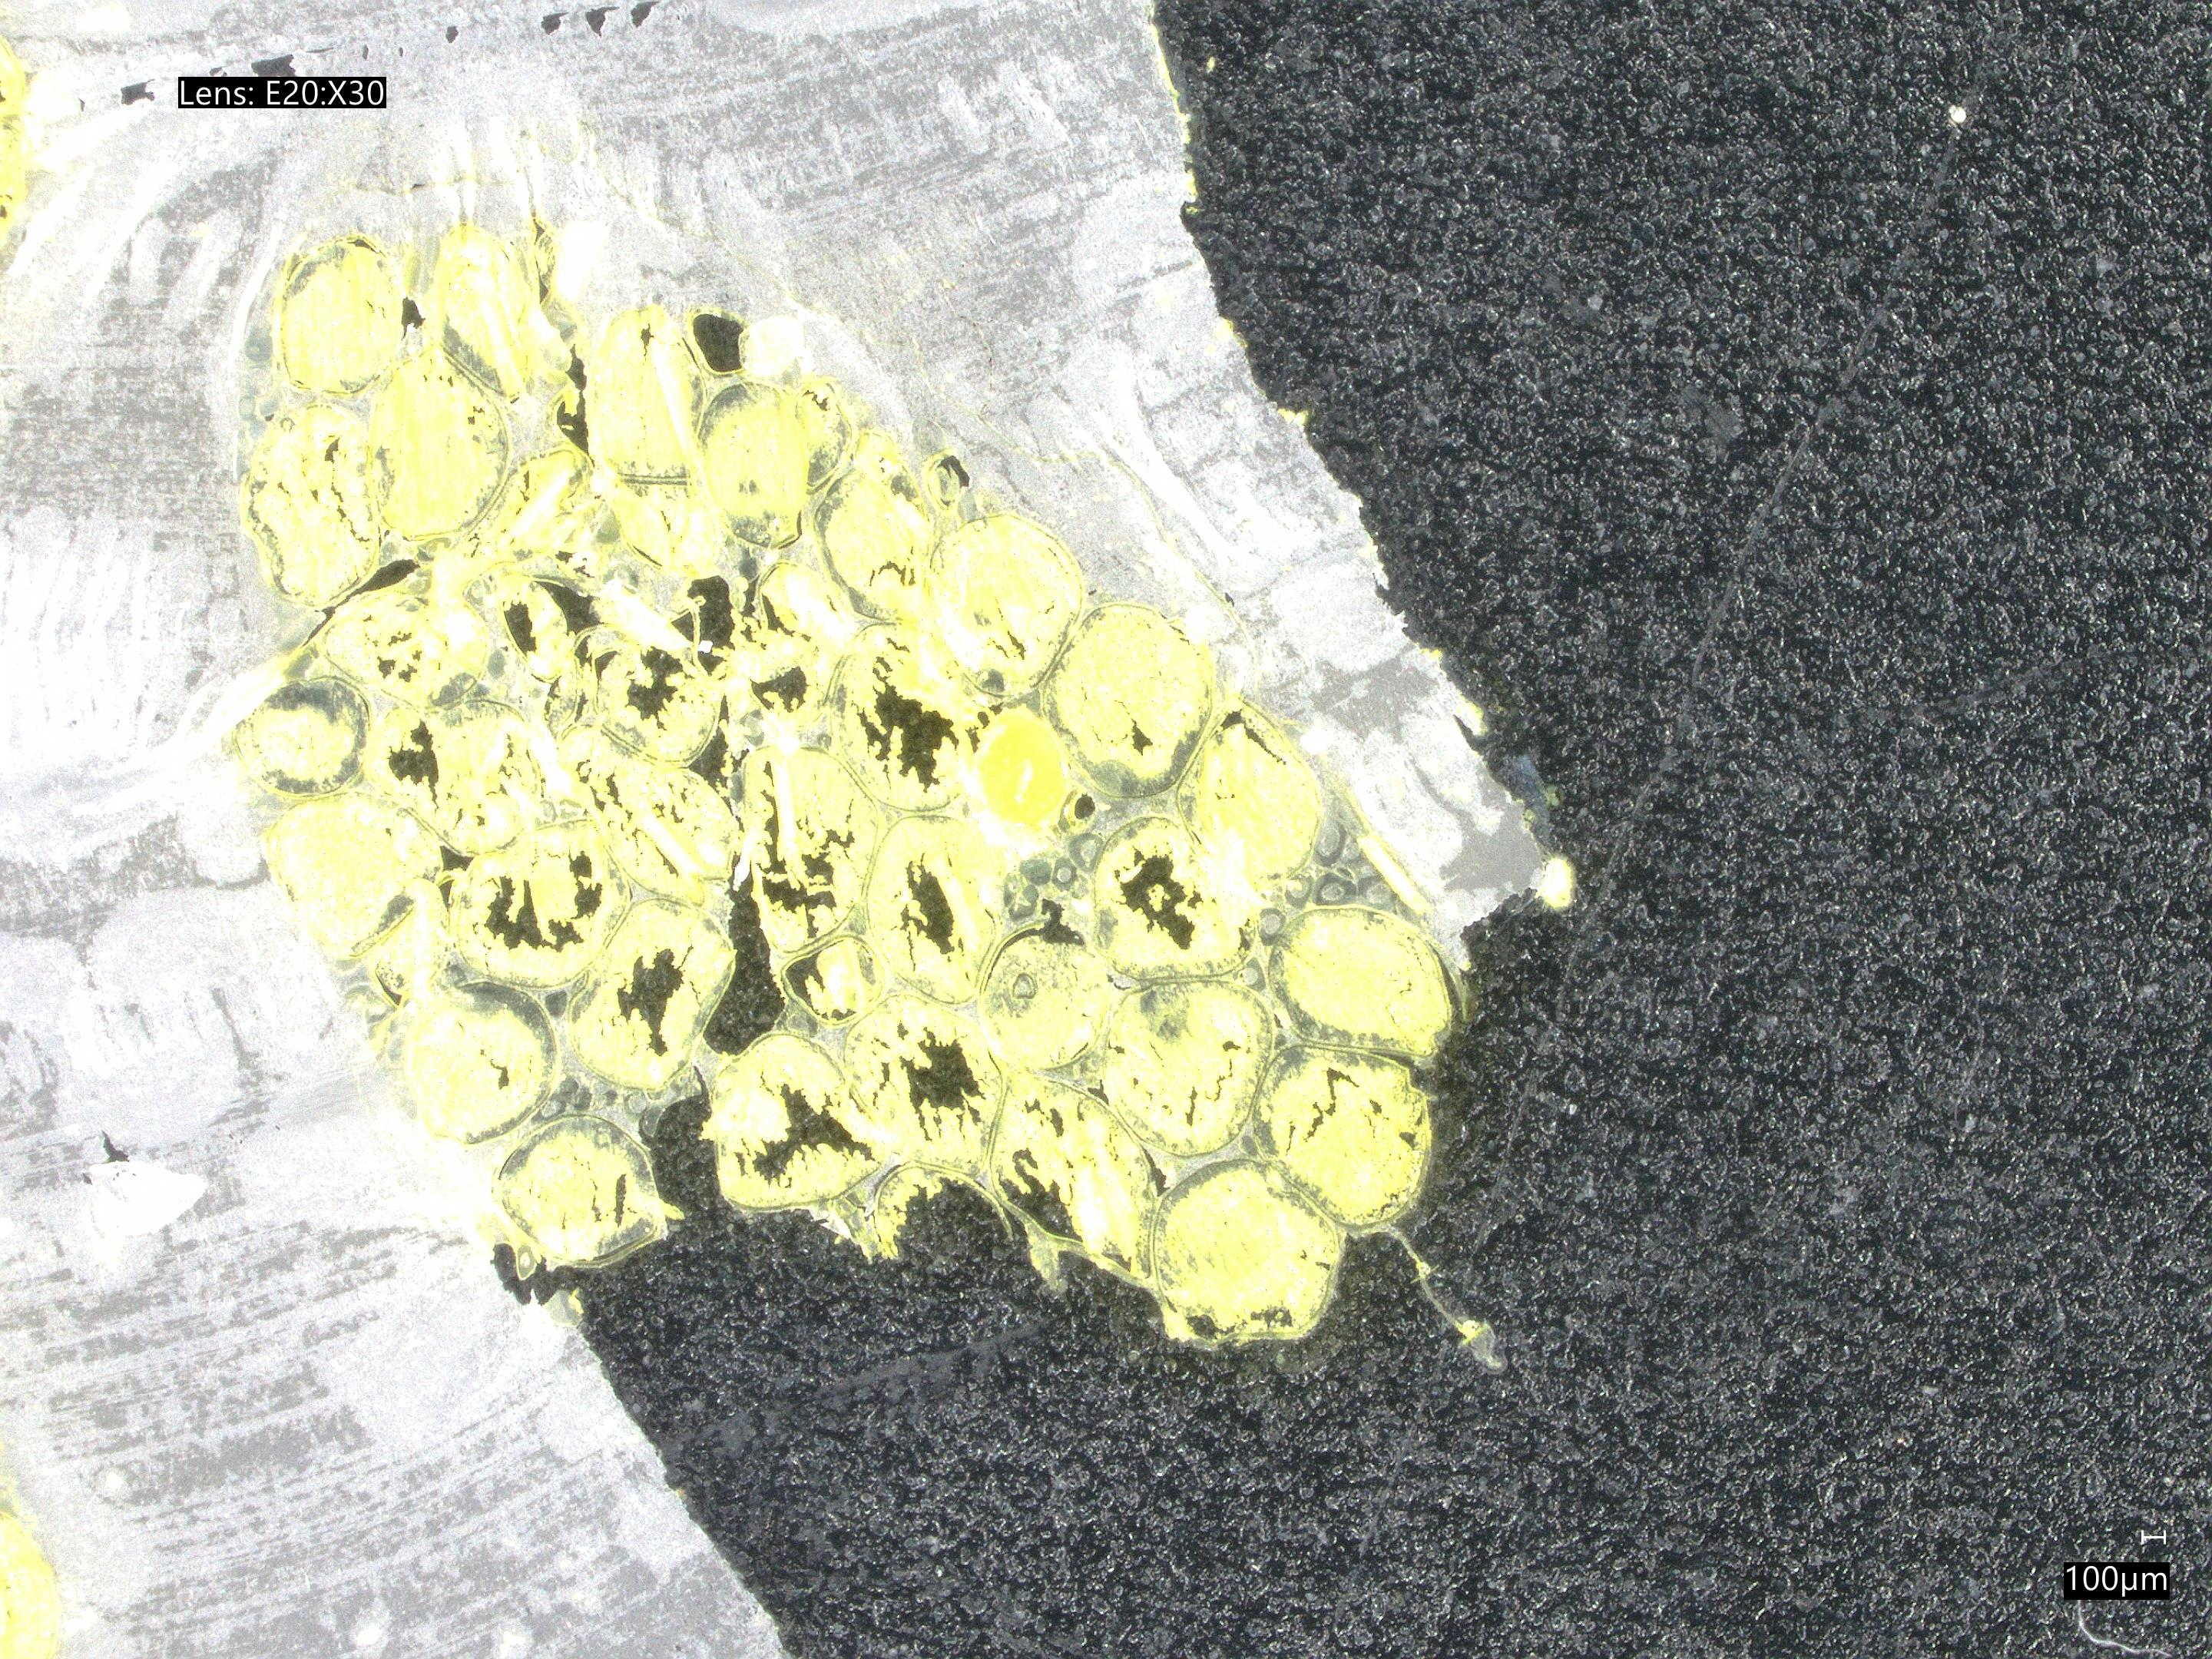
\includegraphics[width=\textwidth]{./fig/fish_lung/other20240313_141858.jpg}
        \caption{other fish lung}
        \label{fig:other_fish_lung}
\end{minipage}
\end{figure}


训练的准确度和损失如\autoref{fig:model5_acc}和\autoref{fig:model5_loss}所示。
\begin{figure}
    \centering
    \begin{minipage}{0.45\textwidth}
        \centering
        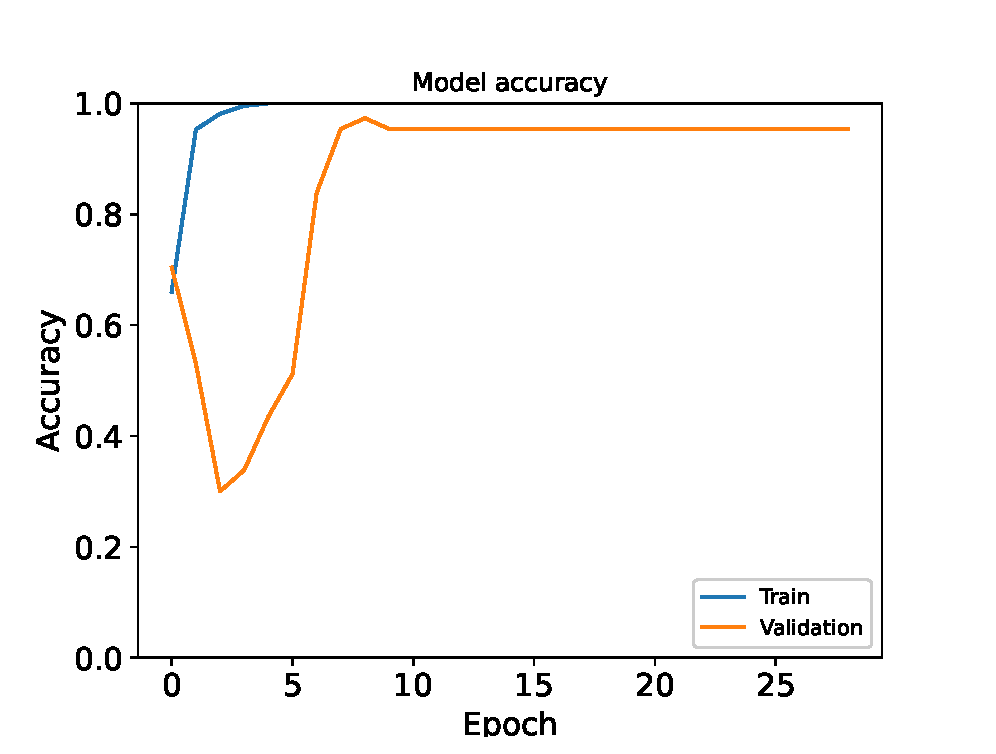
\includegraphics[width=\textwidth]{./fig/fish_lung/accuracy5.eps}
        \caption{Model-5 accuracy}
        \label{fig:model5_acc}
    \end{minipage}
    \begin{minipage}{0.45\textwidth}
        \centering
        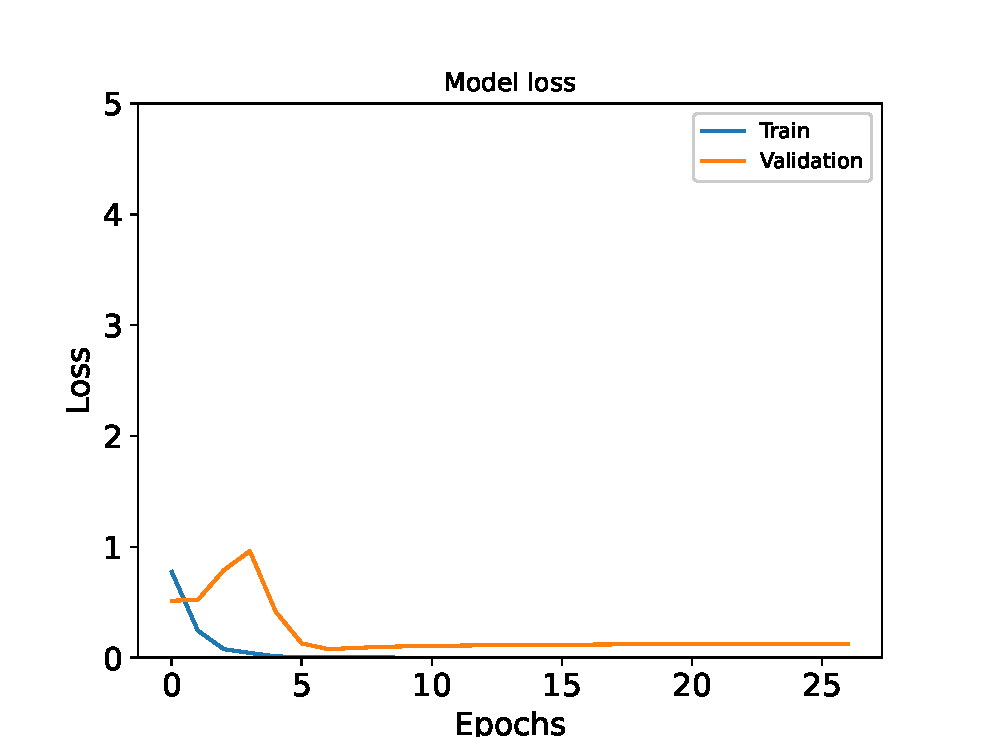
\includegraphics[width=\textwidth]{./fig/fish_lung/loss5.eps}
        \caption{Model-5 loss}
        \label{fig:model5_loss}
    \end{minipage}
\end{figure}

通过观察图片可以得出:
模型5的训练和验证准确度迅速上升并保持在高位,表明模型在这两个数据集上均有良好表现,损失图显示训练损失快速降低并趋于零,而验证损失在初始阶段出现尖峰后迅速降低并稳定,整体来看,这些迹象表明模型具有较好的拟合能力和泛化性能。






% https://ieeexplore.ieee.org/abstract/document/9706974

% https://link.springer.com/chapter/10.1007/978-3-030-33128-3_1

% https://www.sciencedirect.com/science/article/pii/S1120179721000946

% https://scholar.google.com/scholar?hl=zh-CN&as_sdt=0%2C5&q=deep+learning+in+medical+sample&btnG= 参考别人的文章
\FloatBarrier